\documentclass[11pt,twoside]{article}
\usepackage[dvips]{graphicx}
\usepackage{natbib}
\usepackage{fancyhdr,setspace,subfigure,rotate}
\usepackage{amsthm,amssymb,amsmath}
%\usepackage{lineno}
\usepackage{color}
\usepackage{ctable}
\IfFileExists{url.sty}{\usepackage{url}}{\newcommand{\url}{\text}}
\usepackage{sectsty}
\allsectionsfont{\normalsize}
\numberwithin{equation}{section}

\setlength{\oddsidemargin}{0.0in}
\setlength{\evensidemargin}{0.0in}
\setlength{\topmargin}{0.0in}
\setlength{\textheight}{8.5in}
\setlength{\textwidth}{6.25in}
%\setlength{\parskip}{2.0ex}
\setlength{\parindent}{0.2in}
\setlength{\headheight}{14pt}

%\renewcommand{\baselinestretch}{1.2}   % changes \baselineskip to 1.2 x \baselineskip
\DeclareMathOperator*{\argmin}{argmin}

\pagestyle{fancy}
\fancyhead{} % clear all header fields
\fancyhead[CE]{\textit{Boone}}
\fancyhead[CO]{\textit{Data Assimilation Discussion}}
\fancyhead[RE]{\thepage}
\fancyhead[LO]{\thepage}
\lfoot{}
\cfoot{}
\rfoot{}
%\pagenumbering{}

\renewcommand{\headrulewidth}{0pt}

%===================================================================================
\begin{document}
\title{\large \textbf{Data Assimilation Discussion}}
\author{
\normalsize Edward L.~Boone\\ 
\normalsize \textit{Department of Statistical Sciences and Operations Research,} \\
\normalsize \textit{Virginia Commonwealth University,}\\ 
\normalsize \textit{Richmond, VA 23284, USA}\\ 
\normalsize \textit{E-mail: elboone@vcu.edu} \\[0.1in]
}
%\date{March 13, 2014}
\maketitle
\vspace{0.1in}

\hrule
\begin{abstract}
Discussion on Data Assimilation
\end{abstract}
%{\em AMS Subject Classification:} 62F03, 62F15, and 62P10\\
%\\
{\em Keywords:} Data Assimilation 
%in alphabatical order
\vspace{0.1in}
\hrule

%===================================================================================
\section{Introduction}
\label{sect-intro}

\begin{figure}[ht!]
  \begin{center}
   \begin{tabular}{c c}
%\multicolumn{2}{c}{Training} \\ 
    (a) & (b) \\
    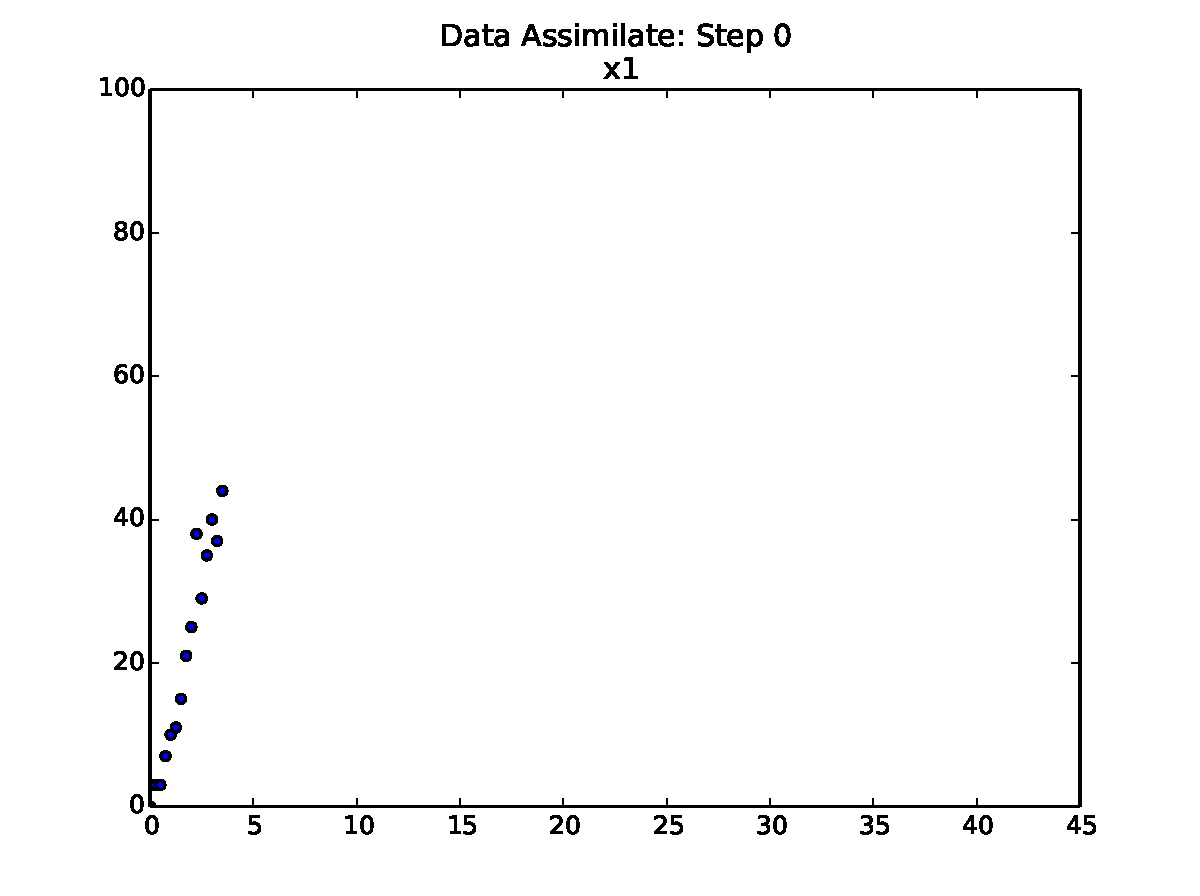
\includegraphics[width=3in]{DSStep0x1.pdf} &
    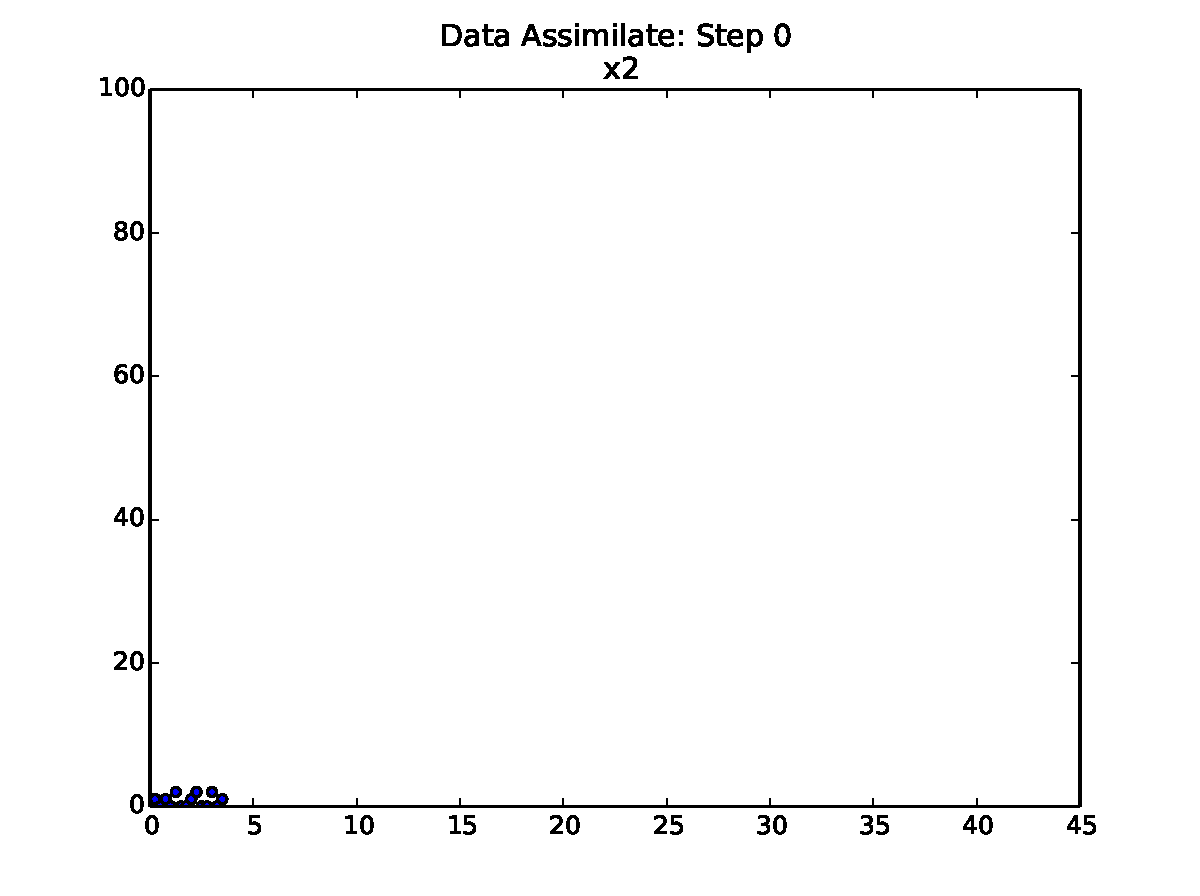
\includegraphics[width=3in]{DSStep0x2.pdf} \\
    (c) & (d) \\
    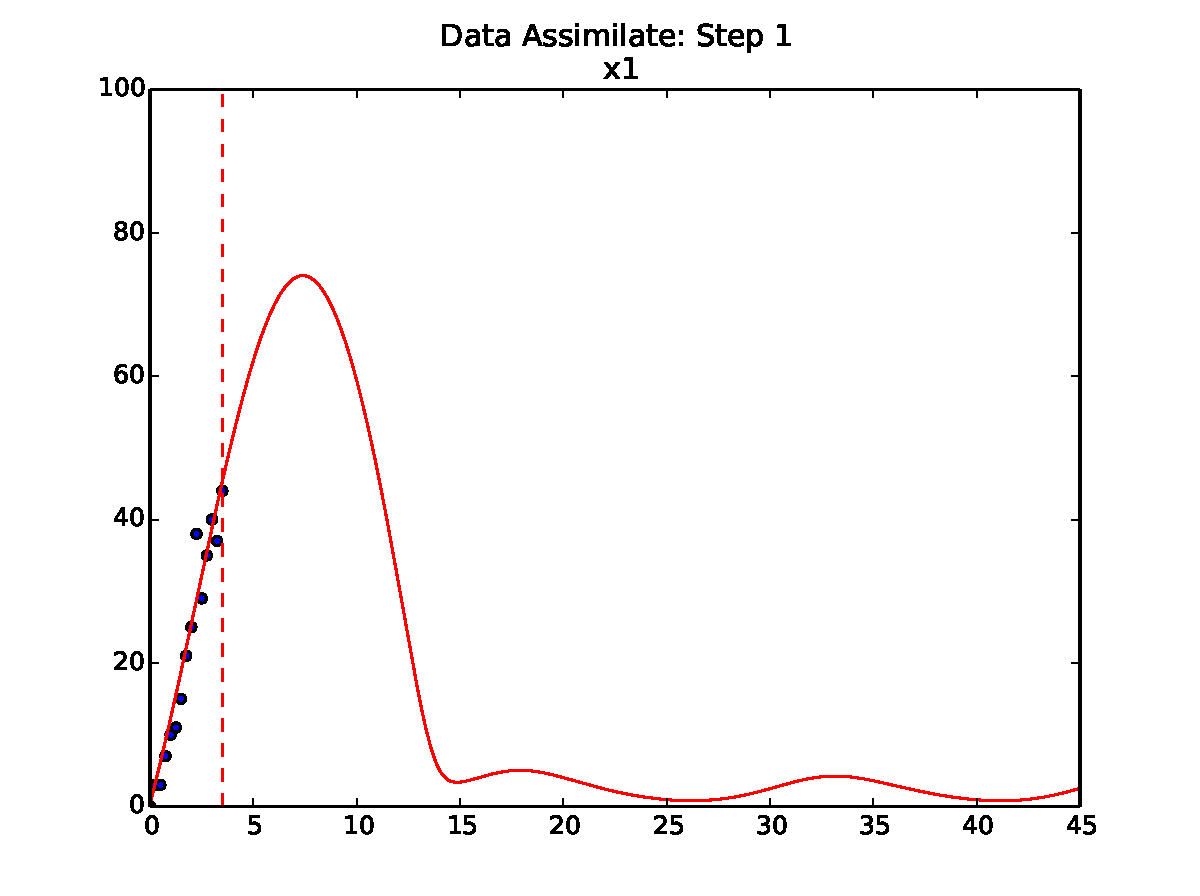
\includegraphics[width=3in]{DSStep1x1.pdf} &
    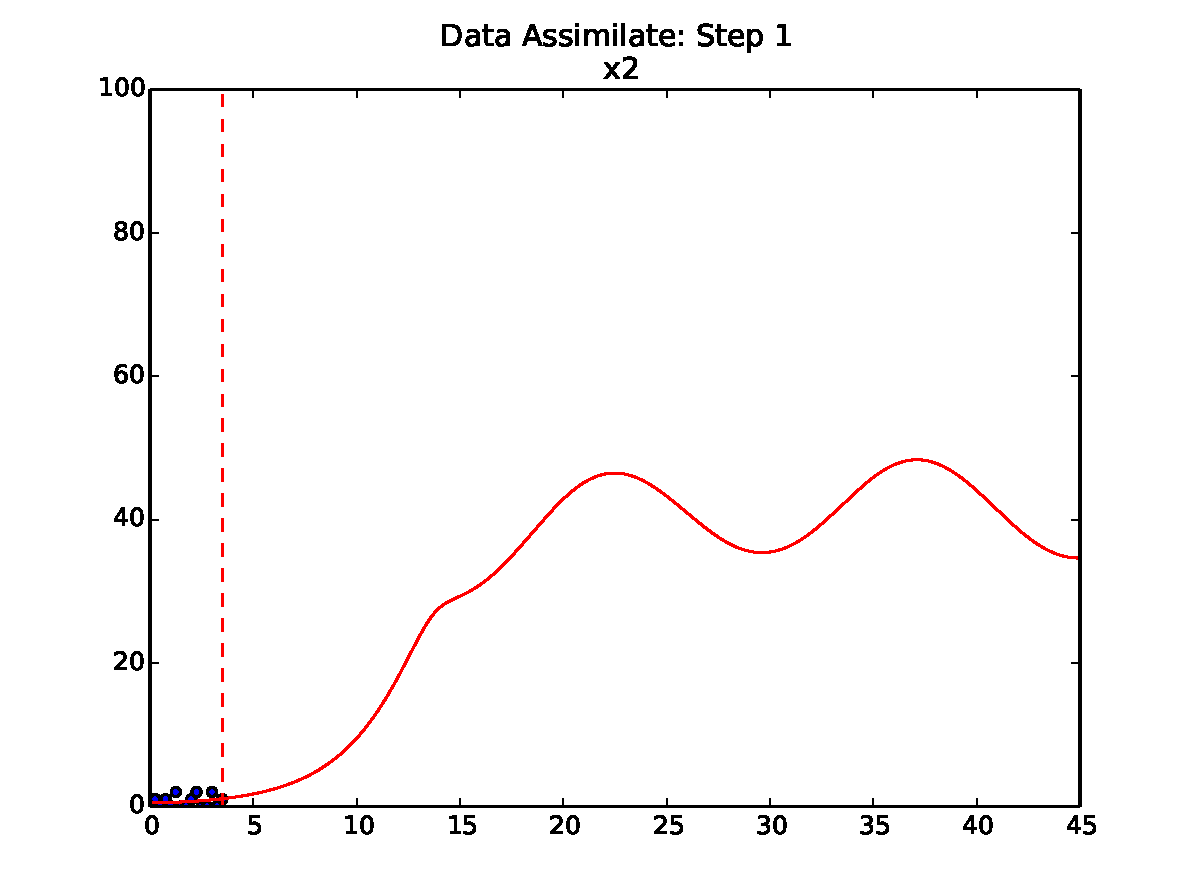
\includegraphics[width=3in]{DSStep1x2.pdf} \\
    (e) & (f) \\
    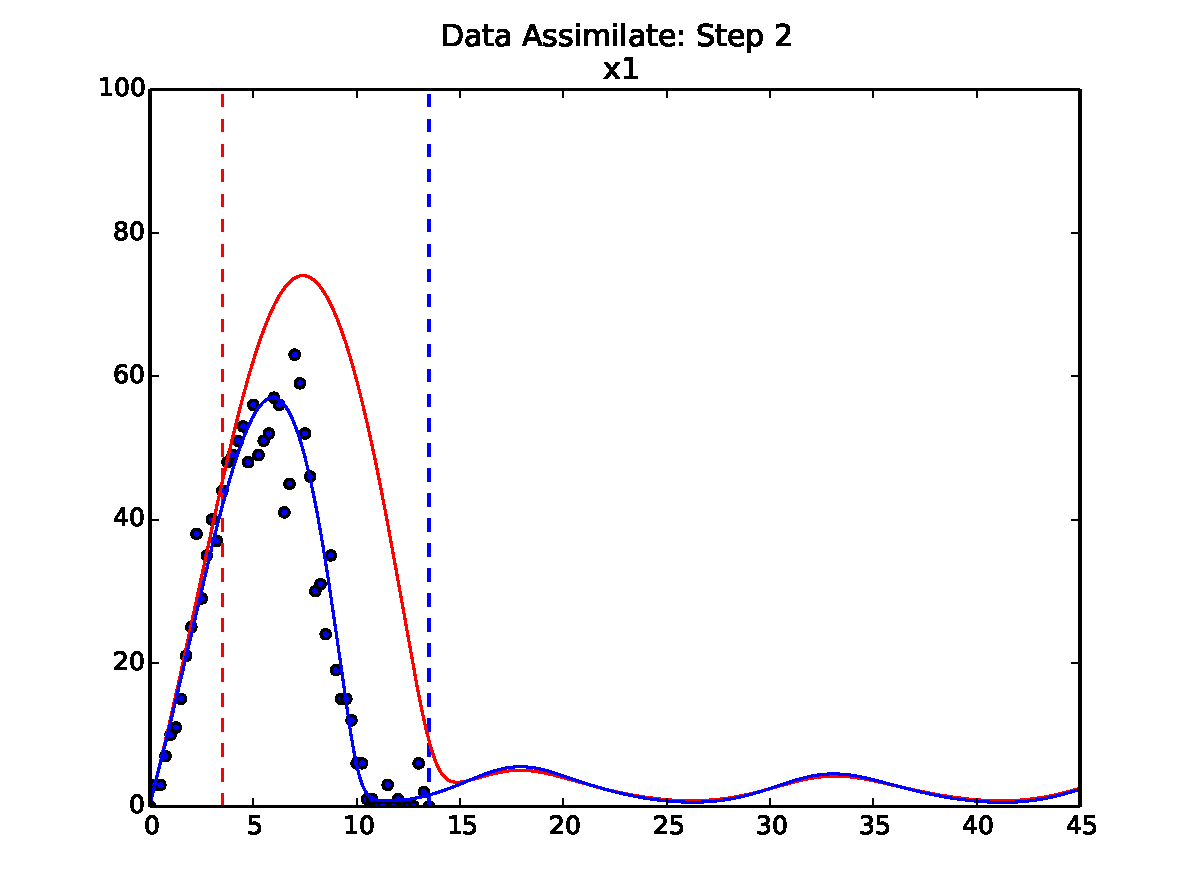
\includegraphics[width=3in]{DSStep2x1.pdf} &
    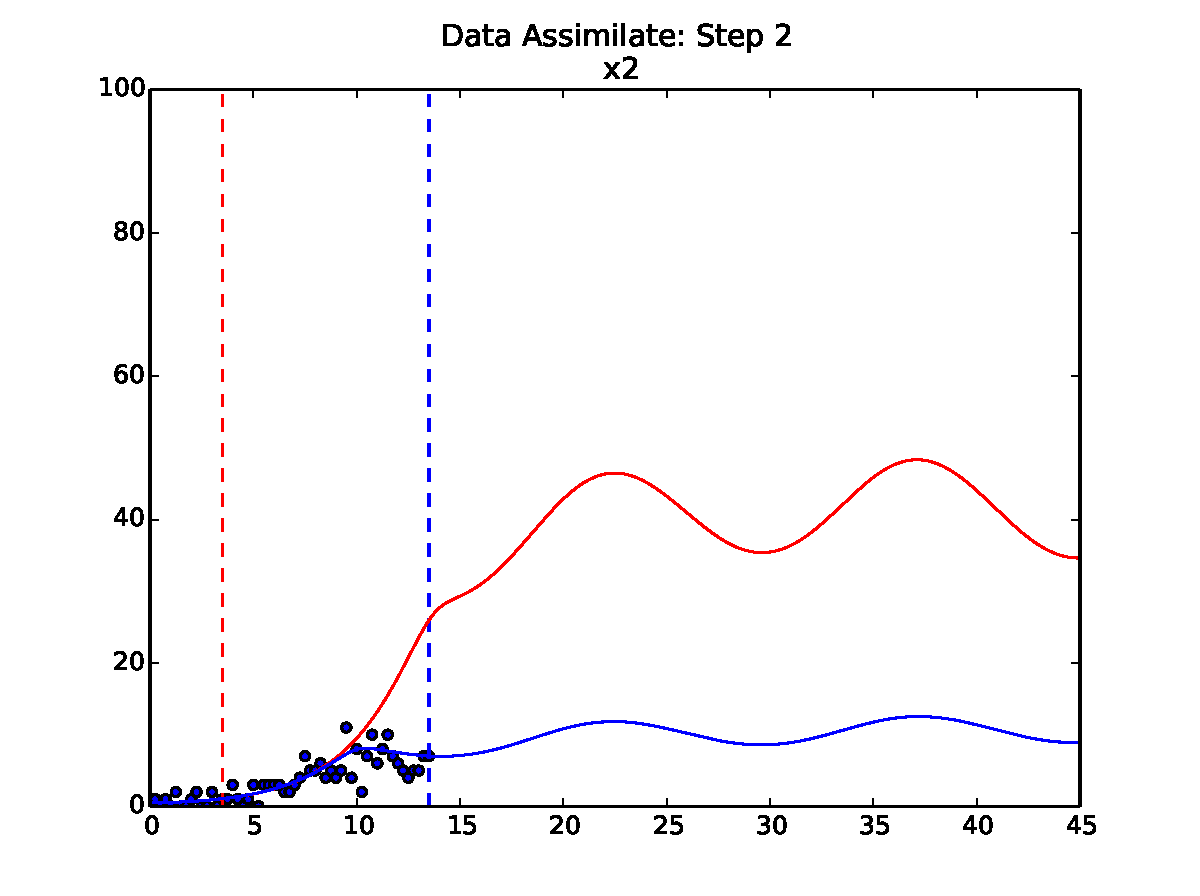
\includegraphics[width=3in]{DSStep2x2.pdf} \\
      \end{tabular}
  \end{center}\caption{ Data for (a) x1, (b) x2 , (c) data with fitted model for x1, (d) data with fitted model for x2, (e) additional data and updated fitted model for x1 and (f) additional data and updated fitted model for x2.}\label{fig:Example1}
\end{figure}



\section*{Acknowledgements}
We thank the opportunities provided by SAMSI. 

\begin{thebibliography}{}
\bibitem[\protect\citeauthoryear{Berntsen, Espelid, and Genz}{Berntsen et al.}{1991}]{berntsen} 
%\bibitem{bern} 
Berntsen, J., Espelid, T.O., and Genz, A. (1991) An Adaptive Algorithm for the Approximate Calculation 
of Multiple Integrals, {\it ACM Transactions on Mathematical Software}, {\bf 17}, 437--451.
\end{thebibliography}


\end{document}




